\begin{frame}{Experiment 5}
\setbeamercovered{invisible}
\fontsize{11pt}{15}\selectfont
\only<1>{\begin{figure}
    \centering
    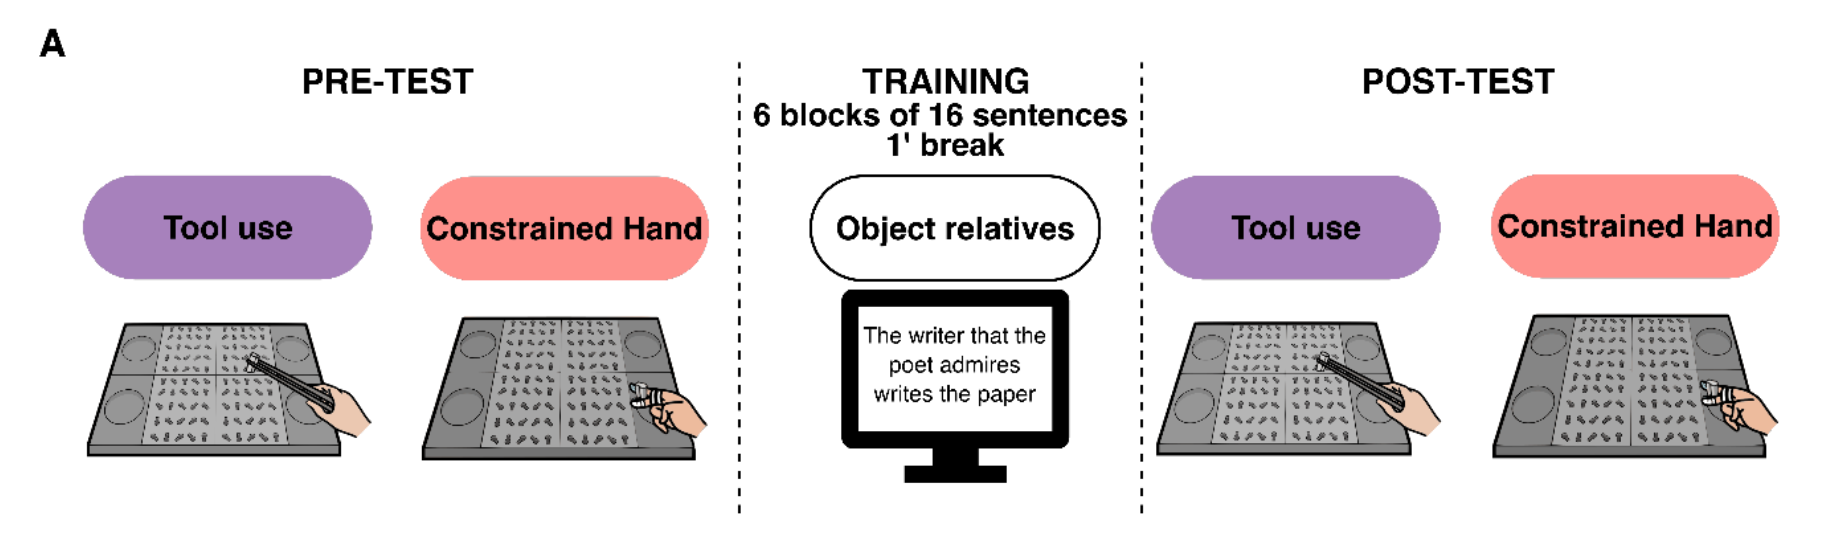
\includegraphics[width=9cm]{images/paper_pics/figS4A.png}
    \caption*{Two groups were tested in entering pegs as fast as possible with the tool (purple) or the constrained hand (red), before and after training with object relative clauses.}
    \label{fig:label12}
\end{figure}}
\pause
\only<2>{{\large\textbf{Results:\\}}
\begin{itemize}
    \item Motor improvement observed after linguistic training with object relatives is \textbf{specific} to \textbf{tool use}.
    \item \textbf{After training}, participants inserted \textbf{more pegs with the tool} than the constrained hand.
\end{itemize}
}



\end{frame}